% Cruise Range Chart - Wheel Pants ON
\begin{figure}[t]
% \addcontentsline{toc}{section}{Figure \ref{Cruise-range} Cruise Range}
\addcontentsline{toc}{section}{CRUISE RANGE}
\begin{center}
\begin{perfhdr}CRUISE RANGE\\
\end{perfhdr}

\begin{minipage}{5in}
  \begin{flushleft}
    CONDITIONS:\\
    Wheel Pants and Gear Leg Fairings ON\\
    43 USG Usable Fuel.\\
    Standard atmosphere.\\
    No wind.\\
    Includes 1.5 USG fuel for start, taxi and takeoff and a 8 USG reserve.\\
    Climb at full power and normal climb speed as defined on the Normal Climb Chart\\
    Lean during climb for best power.\\
    Descend at 180 KTAS at 500 ft/mn (6 nm per 1000 ft).\\
    \end{flushleft}
\end{minipage}\\
\vspace{5ex}
% GNUPLOT: LaTeX picture with Postscript
\begingroup
  \makeatletter
  \providecommand\color[2][]{%
    \GenericError{(gnuplot) \space\space\space\@spaces}{%
      Package color not loaded in conjunction with
      terminal option `colourtext'%
    }{See the gnuplot documentation for explanation.%
    }{Either use 'blacktext' in gnuplot or load the package
      color.sty in LaTeX.}%
    \renewcommand\color[2][]{}%
  }%
  \providecommand\includegraphics[2][]{%
    \GenericError{(gnuplot) \space\space\space\@spaces}{%
      Package graphicx or graphics not loaded%
    }{See the gnuplot documentation for explanation.%
    }{The gnuplot epslatex terminal needs graphicx.sty or graphics.sty.}%
    \renewcommand\includegraphics[2][]{}%
  }%
  \providecommand\rotatebox[2]{#2}%
  \@ifundefined{ifGPcolor}{%
    \newif\ifGPcolor
    \GPcolorfalse
  }{}%
  \@ifundefined{ifGPblacktext}{%
    \newif\ifGPblacktext
    \GPblacktexttrue
  }{}%
  % define a \g@addto@macro without @ in the name:
  \let\gplgaddtomacro\g@addto@macro
  % define empty templates for all commands taking text:
  \gdef\gplbacktext{}%
  \gdef\gplfronttext{}%
  \makeatother
  \ifGPblacktext
    % no textcolor at all
    \def\colorrgb#1{}%
    \def\colorgray#1{}%
  \else
    % gray or color?
    \ifGPcolor
      \def\colorrgb#1{\color[rgb]{#1}}%
      \def\colorgray#1{\color[gray]{#1}}%
      \expandafter\def\csname LTw\endcsname{\color{white}}%
      \expandafter\def\csname LTb\endcsname{\color{black}}%
      \expandafter\def\csname LTa\endcsname{\color{black}}%
      \expandafter\def\csname LT0\endcsname{\color[rgb]{1,0,0}}%
      \expandafter\def\csname LT1\endcsname{\color[rgb]{0,1,0}}%
      \expandafter\def\csname LT2\endcsname{\color[rgb]{0,0,1}}%
      \expandafter\def\csname LT3\endcsname{\color[rgb]{1,0,1}}%
      \expandafter\def\csname LT4\endcsname{\color[rgb]{0,1,1}}%
      \expandafter\def\csname LT5\endcsname{\color[rgb]{1,1,0}}%
      \expandafter\def\csname LT6\endcsname{\color[rgb]{0,0,0}}%
      \expandafter\def\csname LT7\endcsname{\color[rgb]{1,0.3,0}}%
      \expandafter\def\csname LT8\endcsname{\color[rgb]{0.5,0.5,0.5}}%
    \else
      % gray
      \def\colorrgb#1{\color{black}}%
      \def\colorgray#1{\color[gray]{#1}}%
      \expandafter\def\csname LTw\endcsname{\color{white}}%
      \expandafter\def\csname LTb\endcsname{\color{black}}%
      \expandafter\def\csname LTa\endcsname{\color{black}}%
      \expandafter\def\csname LT0\endcsname{\color{black}}%
      \expandafter\def\csname LT1\endcsname{\color{black}}%
      \expandafter\def\csname LT2\endcsname{\color{black}}%
      \expandafter\def\csname LT3\endcsname{\color{black}}%
      \expandafter\def\csname LT4\endcsname{\color{black}}%
      \expandafter\def\csname LT5\endcsname{\color{black}}%
      \expandafter\def\csname LT6\endcsname{\color{black}}%
      \expandafter\def\csname LT7\endcsname{\color{black}}%
      \expandafter\def\csname LT8\endcsname{\color{black}}%
    \fi
  \fi
  \setlength{\unitlength}{0.0500bp}%
  \begin{picture}(7200.00,5040.00)%
    \gplgaddtomacro\gplbacktext{%
      \csname LTb\endcsname%
      \put(1342,704){\makebox(0,0)[r]{\strut{}0}}%
      \csname LTb\endcsname%
      \put(1342,1286){\makebox(0,0)[r]{\strut{}2,000}}%
      \csname LTb\endcsname%
      \put(1342,1867){\makebox(0,0)[r]{\strut{}4,000}}%
      \csname LTb\endcsname%
      \put(1342,2449){\makebox(0,0)[r]{\strut{}6,000}}%
      \csname LTb\endcsname%
      \put(1342,3030){\makebox(0,0)[r]{\strut{}8,000}}%
      \csname LTb\endcsname%
      \put(1342,3612){\makebox(0,0)[r]{\strut{}10,000}}%
      \csname LTb\endcsname%
      \put(1342,4193){\makebox(0,0)[r]{\strut{}12,000}}%
      \csname LTb\endcsname%
      \put(1342,4775){\makebox(0,0)[r]{\strut{}14,000}}%
      \csname LTb\endcsname%
      \put(1474,484){\makebox(0,0){\strut{} 500}}%
      \csname LTb\endcsname%
      \put(2823,484){\makebox(0,0){\strut{} 550}}%
      \csname LTb\endcsname%
      \put(4172,484){\makebox(0,0){\strut{} 600}}%
      \csname LTb\endcsname%
      \put(5520,484){\makebox(0,0){\strut{} 650}}%
      \csname LTb\endcsname%
      \put(6869,484){\makebox(0,0){\strut{} 700}}%
      \put(308,2739){\rotatebox{-270}{\makebox(0,0){\strut{}Altitude (ft)}}}%
      \put(4171,154){\makebox(0,0){\strut{}Cruise Range (NM)}}%
      \put(3227,1373){\rotatebox{77}{\makebox(0,0)[l]{\strut{}75\% Power}}}%
      \put(4576,1727){\rotatebox{76}{\makebox(0,0)[l]{\strut{}65\% Power}}}%
      \put(6060,2158){\rotatebox{76}{\makebox(0,0)[l]{\strut{}55\% Power}}}%
      \put(4172,3874){\makebox(0,0){\strut{}\Large\textcolor{red}{FROM ANALYSIS OF CAFE DATA}\normalsize}}%
      \put(4172,3292){\makebox(0,0){\strut{}\Large\textcolor{red}{PENDING FLIGHT TEST}\normalsize}}%
    }%
    \gplgaddtomacro\gplfronttext{%
    }%
    \gplbacktext
    \put(0,0){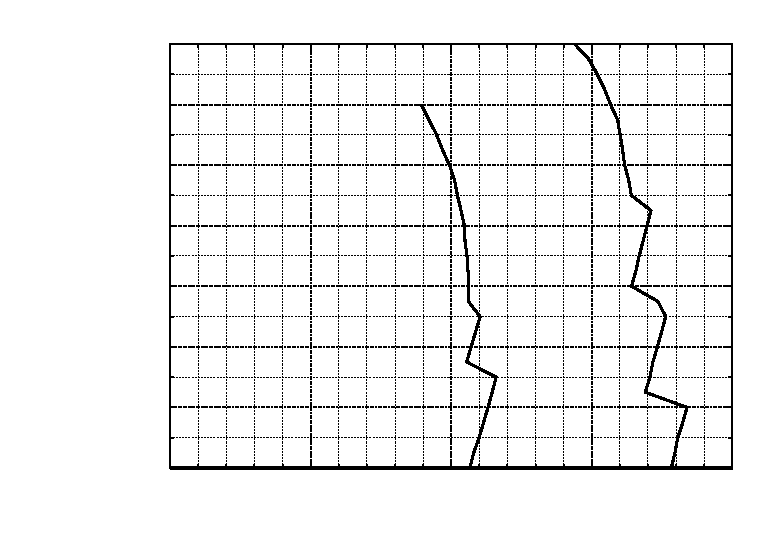
\includegraphics{../graphs/cruise_range}}%
    \gplfronttext
  \end{picture}%
\endgroup
\end{center}  % for gnuplot epslatex, latex or pslatex mode
\caption{Cruise Range}
\label{Cruise-range}
\end{figure}
\clearpage


